\documentclass{article}
\usepackage{chtt-notes}

\usepackage{tikz}
\usetikzlibrary{patterns}

\scribes{Yue Niu and Charles Yuan}
\week{4}
\doXRs

\begin{document}

\maketitle

Thus far in the course, we have covered a typed lambda calculus augmented with inductively defined
positive types such as natural numbers, booleans, products, and sums, as well as how they may be
formulated in a negative fashion. Instead of delving deeper into negatively defined coinductive
types, we will now examine quantification.

\section{Quantification}

Type-level quantification, as seen in System F and its variants, allow us to write types and expressions
containing type variables, which assert validity over all types $\alpha$, or over some type $\alpha$.
\[ \forall X. A \qquad \exists X.A \]

The theory of type polymorphism was largely developed by Gordon, \cite{Milner}, and Wadsworth, and
has been adopted in languages such as ML. It enables innovations such as the polymorphic identity
function:
\[ \texttt{id} : \all{X}{\fn{X}{X}} \]

To begin, consider the following syntax for types, incorporating variables, a positive answer type
\texttt{ans}, functions, and a universal type quantifier.
\[ A \Coloneqq X~|~\texttt{ans}~|~\fn{A_1}{A_2}~|~\all{X}{A} \]

The expressions are defined correspondingly, with a mechanism for type lambdas:
\[ M \Coloneqq x~|~\ap{M_1}{M_2}~|~\lam{x}{A}{M}~|~\tlam{X}{M}~|~\tap{M}{A}~|~\uparrow~|~\downarrow \]

The typing judgment is defined as follows:
\begin{mathpar}
  \inferrule{ }{\hasEF{\Gamma, x : A}{x}{A}}\and
  \inferrule{ }{\hasEF{\Gamma}{\uparrow}{\texttt{ans}}}\and
  \inferrule{ }{\hasEF{\Gamma}{\downarrow}{\texttt{ans}}}\and
  \inferrule{
    \hasEF{\Gamma, x : A_1}{A_2}{M_2}
  }{\hasEF{\Gamma}{\lam{x}{A_1}{M_2}}{\fn{A_1}{A_2}}} \and
  \inferrule{
    \hasEF{\Gamma}{M_1}{\fn{A_1}{A_2}}\\
    \hasEF{\Gamma}{M_2}{A_1}
  }{\hasEF{\Gamma}{\ap{M_1}{M_2}}{A_2}} \and
  \inferrule{
    \hasEF{\Gamma, x}{M}{A}
  }{\hasEF{\Gamma}{\tlam{X}{M}}{\all{X}{A}}} \and
  \inferrule{
    \hasEF{\Gamma}{M}{\all{X}{A}}\\
    \hasTF{\Gamma}{B}
  }{\hasEF{\Gamma}{\tap{M}{B}}{\subst{B}{X}{A}}}
\end{mathpar}

\subsection{Context Splitting}

Now that both expressions and types are allowed to vary, we split the judgment context into two
components: $\Theta$, a finite set of type variables, and $\Gamma$, a finite set of variables as
before. We use both contexts in a judgment, as:
\[ \hasEF{\Theta, \Gamma}{M}{A} \]

\subsection{Erasure}

So far, we have expressed the claim that
\[ M : A~\text{implies}~\bterm{M} \]
that is,
\[(\hasEF{\Gamma}{M}{A}~\text{and}~\hterm{\Gamma}{\gamma})~\text{imply}~\hterm{A}{\hat\gamma(M)} \]

\newcommand{\eraseone}[1]{\ensuremath{{|#1|}^1}}
\newcommand{\erasetwo}[1]{\ensuremath{{|#1|}^2}}
Now that we have type lambdas and variables, we recognize that semantics about expressions should
need to specially account for type lambda abstraction and application. We should instead \emph{erase}
this polymorphic type information before reasoning about hereditary termination, etc. There are
two logical approaches to performing erasure:
\begin{enumerate}
    \item Full erasure. Here, we simply elide all type lambda application and abstraction from
    the expression. We will use the notation \eraseone{M} for this, i.e.:
    \begin{align*}
    \ldots &\\
    \eraseone{\tlam{X}{M}} &= \eraseone{M}\\
    \eraseone{\tap{M}{A}} &= \eraseone{M}
    \end{align*}
    where every other erasure rule simply erases each component of $M$ in the expected fashion.
    \item Delayed erasure. Here, we replace type lambdas with classical lambdas and type applications
    with classical applications. The expression argument is a dummy, and given a choice for its type
    we arbitarily select the answer type (and $\uparrow$ as its value).
    \begin{align*}
    \ldots &\\
    \erasetwo{\tlam{X}{M}} &= \alam{\erasetwo{M}}\\
    \erasetwo{\tap{M}{A}} &= \ap{\erasetwo{M}}{(\uparrow)}
    \end{align*}
\end{enumerate}

Note that in full erasure, it is possible for a value (a type lambda) to become a non-value after
erasure (the body of the lambda), whereas this is impossible in delayed erasure. Allowing values
to become non-values has negative consequences later, and can make the result unsound. From now we
will use the notation for erasure, $\erase{M}$, to refer to delayed erasure $\erasetwo{M}$.

\section{Termination}

Our goal is to prove, for the language augmented with quantifiers:
\[ M : A \implies \bterm{\erase{M}} \]

Let us begin with the obvious attempt. We will use hereditary termination, $\hterm{A}{M}$, taking
erasure into account.

\begin{proofattempt}
\begin{itemize}
\item $\hterm{x}{M}$.
      We're not sure how to proceed here yet. Moving on for a moment...

\item $\hterm{\texttt{ans}}{M} \iff \stepbs{M}{\uparrow}$ or $\stepbs{M}{\downarrow}$.
      This is straightforward.

\item $\hterm{\fn{A_1}{A_2}}{M} \iff \hterm{A_1}{M_1} \implies \hterm{A_2}{\ap{M}{M_2}}$.
      We've seen this before.

\item $\hterm{\all{X}{A}}{M} \iff $ for all closed $B$, we have $\hterm{\subst{B}{X}{A}}{\tap{M}{B}}$.

      Let's think about this case. First, observe that $\tap{M}{B}$ should actually be written as
      $M(\downarrow)$, due to erasure. Next, there is a central issue!
      The substitution of $B$ into $A$ may result in a type that is structurally larger than
      \all{X}{A}. For example, let $B=\fn{(\all{X}{\fn{X}{A}})}{(\all{X}{\fn{X}{X}})}$, which
      clearly will not yield a result that is smaller than $A$. This scheme is \emph{not inductive},
      and it \textcolor{red}{fails}.
\end{itemize}
\end{proofattempt}

At this point, we may be frustrated enough to try a desperate move: defining some alternative
measure of size that means the substitution may not become larger than $A$, and would allow us to
move forward with the previous attempt. This would be difficult, as we would not know where to
start in defining such a measure, and it likely does not exist at all.

\subsection{Next Attempt}

\newcommand{\htermFFm}[4]{\ensuremath{\mathsf{HT}_{#1}(#2)[#3 : #4]}}

Having been thwarted by the substitution, let us try to factor it out. Define
\[ \htermFFm{A}{M}{\delta}{\Theta} \]

as the hereditary termination of $M$ at $A$ with a \emph{closing type substitution} $\delta$ with respect
to $\Theta$. Now $A$ can be open (which also allows us to deal with the first case from earlier).
In particular, \hasTF{\Theta}{A}. We restate the problematic cases from before:

\begin{itemize}
    \item $\htermFFm{X}{M}{\delta}{\Theta} \iff \hterm{\delta(X)}{M}$.

    This relates the new definition to the old one for type variables, given some closing substitution.

    \item $\htermFFm{\all{X}{A}}{M}{\delta}{\Theta} \iff $ for all closed $B$, we have
          $\htermFFm{A}{M(\downarrow)}{\delta[X \mapsto B]}{\Theta, X}$.

    Now, we allow $X$ to be free in $A$, and record the substitution and $X$ into the context.
    Surely the proof will go through this time?
\end{itemize}

As pleased as we are that we have reorganized the proof, have we really done anything? $B$ is still
a menace as before, and even if we first allow $X$ to be free, eventually we must attempt to close
over it, at which point $B$ resurfaces. We must find some way of truly ridding ourselves of it.

\subsection{A Step Further}

Here is an idea: instead of dealing with $B$ directly, define some \emph{interpretation} of a type
variable. Namely, try:
\[ \htermFF{A}{M}{\delta}{\eta}{\Theta} \]

where $\eta$ is an interpretation, or a set of predicates, of variables, given $\delta$, and
$\eta(X)$ is an interpretation of $X$.
From here on, when $\Theta$ is clear from context we will leave it out.

We restate the cases again:
\begin{itemize}
\item $\htermF{X}{M}{\delta[X\mapsto A]}{\eta[X\mapsto T]} \iff T(M)$, where $T$ is a predicate.
      Letting $\eta' = \eta[X \mapsto T]$, we have $T = \eta'(X)$.

\item $\htermF{\all{X}{A}}{M}{\delta}{\eta} \iff $ for all closed $B$, we have
      $\htermF{A}{M(\downarrow)}{\delta[M \mapsto B]}{\eta[X \mapsto \htermF{B}{-}{\delta}{\eta}]}$.

      So the predicate we wish to use is \htermF{B}{-}{\delta}{\eta}, which we denote the
      \emph{standard interpretation} of $B$. In the proof checking, we eventually check $X$ for
      hereditary termination under $B$.
\end{itemize}

We now seem to be much closer, but the proof is still flawed because checking \htermF{B}{-}{\delta}{\eta}
is still not inductive. This framework requires only one final leap before it is correct. The final
leap is a statement not only about our claim, but about the logic in which we are trying to prove it!

\subsection{A Leap of Faith}

% TODO: I don't know if the terminology is correct here. I'm a bit confused myself as to what
% order each step is working on, how type, type candidate, predicate, and (non)standard interpretation
% relate to each other.

We said that \htermF{B}{-}{\delta}{\eta} is the standard interpretation of $B$, and that checking
it is not inductive in nature. Throughout this whole time we have been pestered by the fact that
we need to pick some specific $B$, and admit that it may be larger than $A$ in the first place.
For every type $B$ there is a corresponding standard interpretation that may be impossible to check.
That leaves the question open: do there exist non-standard interpretations?

% TODO: what parts of this are actually red? What do the Ts mean, and does the predicate HT
% belong inside the circle?

\begin{center}
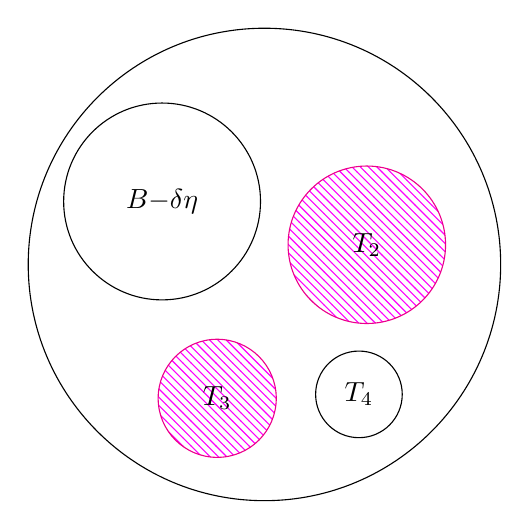
\begin{tikzpicture}[scale=0.5]
\draw (-3.8,-1) circle (6cm);
\draw (-6.4,0.6) circle (2.5cm);
\draw [pattern=north west lines, pattern color=magenta, draw=magenta] (-1.2,-0.5) circle (2cm);
\draw [pattern=north west lines, pattern color=magenta, draw=magenta] (-5.0,-4.4) circle (1.5cm);
\draw (-1.4,-4.3) circle (1.1cm);
\draw (-6.4,0.6) node[anchor=center] {$\htermF{B}{-}{\delta}{\eta}$};
\draw (-1.2,-0.5) node[anchor=center] {$T_2$};
\draw (-5.0,-4.4) node[anchor=center] {$T_3$};
\draw (-1.4,-4.3) node[anchor=center] {$T_4$};
\end{tikzpicture}
\end{center}

% TODO: properly define type candidate

% The diagram above is a depiction of predicates we may wish to use within the interpretation.
% Each circle is the standard interpretation of a type. Some of these circles, indicated in red,
% are hereditary termination conditions we are able to show, whereas some, such as \htermF{B}{-}{\delta}{\eta},
% are unable to be shown directly. But since each condition is merely a predicate on an expression,
% we may indirectly obtain \htermF{B}{-}{\delta}{\eta} by simply taking the \emph{set of all types}.
% The set of all types is not a type. Logically, we must accept quantification over types, which is
% a higher-order comprehension principle.

% TODO: have we been assuming second-order all along?
% TODO: more on Godel (completeness and incompleteness)

Let's step back for a minute. Types themselves are ``sets'' (quantifications) over terms.
Previously we proved the termination of G\"odel's T using the hereditary termination predicates,
which are second-order over terms. According to G\"odel's second incompleteness theorem, Peano
arithmetic (and System T, which contains it) cannot prove its own consistency (computationally
speaking, its termination), so the second-order proof was the best we could do.

Now, System F operates on types the way that System T operates on terms. It has become clear that
to prove termination for System F requires us to move one order higher, to third-order comprehension.
We must produce the set of all type candidates in order to finish the proof, which can only be
done in third-order logic.

With this machinery in place, we are finally ready to redefine the problematic case one last time:

$\htermF{\all{X}{A}}{M}{\delta}{\eta} \iff $ for all closed $B$, for all type candidates $T$,
$\htermF{A}{M(\downarrow)}{\delta[X \mapsto B]}{\eta[X \mapsto T]}$.

Here, we quantify over all type candidates, among which is $T_B$, the type candidate corresponding
to the interpretation of $B$. Note the consequence of this claim on the nature of a polymorphic
computation. For an expression to be polymorphic it must be uniform in \emph{non-expressible properties}
of the system. Some of these properties, like quantification over all type candidates, can only
be stated in a higher-order logic.

\section{Girard's Method}

Recall hereditary termination we discovered through several trials:
\[
\htermFF{A}{M}{\delta}{\eta}{\Theta}
\]
Read as $M$ is hereditarily terminating at $A$, where $delta$ is a closing type variable substitution and $\eta$ is
a candidate assingment, all with respect to $\Theta$. Since it's usually clear from context, we drop $\Theta$ unless it's
required.

To make precise the argument of type candidates, we need to make precise what they mean:

\emph{Type candidates} are any collection $\mathcal{C}$ of \emph{closed, erased} terms such that:
\begin{enumerate}
\item $\mathcal{C}$ is closed under head expansion, and possibly
\item $T \in \mathcal{C}$ and $T(M) \implies \bterm{M}$
\end{enumerate}

Before presenting the FTLR for system F, we will need the following lemma:
\begin{lemma}[Compositionality]\label{lem:comp}
$\htermF{[A/X]B}{M}{\delta}{\eta}$ iff $\htermF{B}{M}{\delta[X \mapsto A]}{\eta[X \mapsto \htermF{A}{-}{\delta}{\eta}]}$
\end{lemma}

\begin{proof}
Induction on $B$.
\begin{itemize}
\setlength\itemsep{1em}
\item $B = X$\\
For the forward direction, suppose $\htermF{[A/X]X}{M}{\delta}{\eta}$. We need to show that
$\htermF{X}{M}{\delta[X \mapsto A]}{\eta[X \mapsto \htermF{A}{-}{\delta}{\eta}]}$. By definition, it sufficese to show
$(\eta[X \mapsto \htermF{A}{-}{\delta}{\eta}])(X)(M)$, or that $\htermF{A}{M}{\delta}{\eta}$, which follows from the
assumption.\\

For the backward direction, suppose $\htermF{X}{M}{\delta[X \mapsto A]}{\eta[X \mapsto \htermF{A}{-}{\delta}{\eta}]}$.
We need to show that $\htermF{[A/X]X}{M}{\delta}{\eta}$, or $\htermF{A}{M}{\delta}{\eta}$, which follows by unfolding
the assumption.

\item $B = X'$ where $X \ne X'$\\
For the forward direction, suppose $\htermF{[A/X]X'}{M}{\delta}{\eta}$. We need to show that
$\htermF{X'}{M}{\delta[X \mapsto A]}{\eta[X \mapsto \htermF{A}{-}{\delta}{\eta}]}$. By definition, it sufficese to show
$(\eta[X \mapsto \htermF{A}{-}{\delta}{\eta}])(X')(M)$. Since $ X \ne X'$,
it suffices to show $\eta(X')(M)$, which holds by assumption. \\

For the backward direction, suppose $\htermF{X'}{M}{\delta[X \mapsto A]}{\eta[X \mapsto \htermF{A}{-}{\delta}{\eta}]}$.
We need to show that $\htermF{[A/X]X'}{M}{\delta}{\eta}$, or $\htermF{X'}{M}{\delta}{\eta}$. By definition, it suffices
to show that $\eta(X')(M)$. By assumption, we know $(\eta[X \mapsto \htermF{A}{-}{\delta}{\eta}])(X')(M)$ holds. Since
$X \ne X'$, $(\eta[X \mapsto \htermF{A}{-}{\delta}{\eta}])(X') = \eta(X')$, and we have that $\eta(X')(M)$ holds.

\item $B = \fn{A_1}{A_2}$\\
For the forward direction, suppose $\htermF{[A/X]B}{M}{\delta}{\eta}$. We need to show that
$\htermF{B}{M}{\delta[X \mapsto A]}{\eta[X \mapsto \htermF{A}{-}{\delta}{\eta}]}$.
Suppose $\htermF{A_1}{N}{\delta[X \mapsto A]}{\eta[X \mapsto \htermF{A}{-}{\delta}{\eta}]}$. It suffices to show
then $\htermF{A_2}{\ap{M}{N}}{\delta[X \mapsto A]}{\eta[X \mapsto \htermF{A}{-}{\delta}{\eta}]}$.
By IH, we have $\htermF{[A/X]XA_1}{N}{\delta}{\eta}$. Further, from assumption we get
$\htermF{\fn{[A/X]A_1}{[A/X]A_2}}{M}{\delta}{\eta}$. By the definition of hereditary termination, we get
$\htermF{[A/X]A_2}{\ap{M}{N}}{\delta}{\eta}$, and the result follows from the IH.

For the backward direction, suppose
$\htermF{\fn{A_1}{A_2}}{M}{\delta[X \mapsto A]}{\eta[X \mapsto \htermF{A}{-}{\delta}{\eta}]}$.
We need to show that $\htermF{[A/X]\fn{A_1}{A_2}}{M}{\delta}{\eta}$,
or $\htermF{\fn{[A/X]A_1}{[A/X]A_2}}{M}{\delta}{\eta}$. Suppose $\htermF{[A/X]A_1}{N}{\delta}{\eta}$.
It suffices to show $\htermF{[A/X]A_2}{\ap{M}{N}}{\delta}{\eta}$. By IH, we have
$\htermF{A_1}{N}{\delta[X \mapsto A]}{\eta[X \mapsto \htermF{A}{-}{\delta}{\eta}]}$.
Along with the assumption, we get $\htermF{A_2}{\ap{M}{N}}{\delta[X \mapsto A]}{\eta[X \mapsto \htermF{A}{-}{\delta}{\eta}]}$, and the result follows from IH.

\item $B = \all{Z}{B'}$\\
For the forward direction, suppose $\htermF{[A/X]\all{Z}{B'}}{M}{\delta}{\eta}$. We need to show that
$\htermF{\all{Z}{B'}}{M}{\delta[X \mapsto A]}{\eta[X \mapsto \htermF{A}{-}{\delta}{\eta}]}$. Let $C$ be a closed type,
and $T$ a type candidate. Letting $\delta' = \delta[X \mapsto A]$ and
$\eta' = \eta[X \mapsto \htermF{A}{-}{\delta}{\eta}]$, it sufficese to show
$\htermF{B'}{\ap{\erase{M}}{\downarrow}}{\delta'[Z \mapsto C]}{\eta'[Z \mapsto T]}$. By the assumption (and
capture-avoiding substitution), we have $\htermF{\all{Z}{[A/X]B'}}{M}{\delta}{\eta}$.
Now instantiate the RHS definition with $C$ and $T$, obtaining
$\htermF{[A/X]B'}{\ap{\erase{M}}{\downarrow}}{\delta[Z \mapsto C]}{\eta[Z \mapsto T]}$.
Let $\delta'' = \delta[Z \mapsto C]$ and $\eta'' = \eta[Z \mapsto T]$. By IH, we have
$\htermF{B'}{\ap{\erase{M}}{\downarrow}}{\delta''[X \mapsto A]}{\eta''[X \mapsto \htermF{A}{-}{\delta''}{\eta''}]}$,
which is what was needed. \footnote{ is the interpretation of $Z$ irrelevant when considering $A$?}\\

For the backward direction, suppose
$\htermF{\all{Z}{B'}}{M}{\delta[X \mapsto A]}{\eta[X \mapsto \htermF{A}{-}{\delta}{\eta}]}$.
We need to show that $\htermF{[A/X]\all{Z}{B'}}{M}{\delta}{\eta}$, or $\htermF{\all{Z}{[A/X]B'}}{M}{\delta}{\eta}$.
Let $C$ be a closed type, and $T$ a type candidate. By definition, it suffices
to show $\htermF{[A/X]B'}{\ap{\erase{M}}{\downarrow}}{\delta[Z \mapsto C]}{\eta[Z \mapsto T]}$.
Instantiating the assumption with $C$ and $T$, we have $\htermF{B'}{\ap{\erase{M}}{\downarrow}}{\delta[X \mapsto A][Z \mapsto C]}{\eta[X \mapsto \htermF{A}{-}{\delta}{\eta}][Z \mapsto T]}$.
By IH, we have $\htermF{[A/X]B'}{\ap{\erase{M}}{\downarrow}}{\delta[Z \mapsto C]}{\eta[Z \mapsto T]}$. \footnote{There needs to be a weakening of the interpretation in order to apply the IH.}
\end{itemize}
\end{proof}

\begin{lemma}[Head expansion]\label{lem:head_exp}
If $\hasTF{\Theta}{A}$, $\delta : \Theta$, $\eta : \Theta$, then $\htermF{A}{-}{\delta}{\eta}$ is a type candidate.
\end{lemma}
\begin{proof}
Induction on $A$.
\begin{itemize}
\setlength\itemsep{1em}
\item $A = X$\\
Suppose $\htermF{A}{M'}{\delta}{\eta}$ and $\step{M}{M'}$. We need to show that $\htermF{A}{M}{\delta}{\eta}$.
By assumption, we have $\eta(X)(M')$. Since $\eta$ is a candidate assignment, $\eta(X)$ is closed under head expansion,
and so $\eta(X)(M)$ holds.
\item $A = \fn{A_1}{A_2}$\\
Suppose $\htermF{\fn{A_1}{A_2}}{M'}{\delta}{\eta}$ and $\step{M}{M'}$.
We need to show that $\htermF{\fn{A_1}{A_2}}{M}{\delta}{\eta}$. Suppose $\htermF{A_1}{N}{\delta}{\eta}$.
It suffices to show that $\htermF{A_2}{\ap{M}{N}}{\delta}{\eta}$. Instantiating the assumption, we get
$\htermF{A_2}{\ap{M'}{N}}{\delta}{\eta}$. Since $\step{\ap{M}{N}}{\ap{M'}{N}}$, by IH, we have our result.
\item $A = \all{X}{B}$\\
Suppose $\htermF{\all{X}{B}}{M'}{\delta}{\eta}$ and $\step{M}{M'}$.
We need to show $\htermF{\all{X}{B}}{M}{\delta}{\eta}$. Let $C$ be a closed type, $T$ a type candidate.
It suffices to show $\htermF{B}{\ap{\erase{M}}{\downarrow}}{\delta[X \mapsto C]}{\eta[X \mapsto T]}$.
Instantiating the assumption with $C$ and $T$, we have
$\htermF{B}{\ap{\erase{M'}}{\downarrow}}{\delta[X \mapsto C]}{\eta[X \mapsto T]}$.
Since $\step{\ap{\erase{M}}{\downarrow}}{\ap{\erase{M'}}{\downarrow}}$, by IH, we have our result.
\end{itemize}
\end{proof}

\begin{theorem}[FTLR for System F]
If $\hasEF{\Theta;\Omega}{M}{A}$, and
\begin{enumerate}
\item $\delta : \Theta$ is a closing type substitution
\item $\eta : \Theta$ is a candidate assignment
\item $\gamma : \cdot \to \Gamma$ is a closig term substitution
\item $\htermF{\Gamma}{\gamma}{\delta}{\eta}$
\end{enumerate}
then $\htermF{A}{\hat\gamma(\erase{M})}{\delta}{\eta}$.
\end{theorem}

\begin{proof}
Induction on typing.
\begin{itemize}
\setlength\itemsep{1em}
\item $\inferrule{
  \hasEF{\Theta, X; \Gamma}{M}{B}
  }{
  \hasEF{\Theta; \Gamma}{\tlam{X}{M}}{\all{X}{B}}
  }$\\
Fix $\delta : \Theta, \eta : \Theta$ and $\htermF{\Gamma}{\gamma}{\delta}{\eta}$. We need to show that
$\htermFF{\all{X}{B}}{\hat\gamma(\erase{\tlam{X}{M}})}{\delta}{\eta}{\Theta}$, or that
$\htermFF{\all{X}{B}}{\alam{\hat\gamma(\erase{M})}}{\delta}{\eta}{\Theta}$.
Let $C$ be a closed type, $T$ a type candidate,
$\delta' = \delta[X \mapsto C]$, $\eta' = \eta[X \mapsto T]$, and $\Theta' = \Theta,X$.
We need to show that $\htermFF{B}{\ap{\alam{\hat\gamma(\erase{M})}}{\downarrow}}{\delta'}{\eta'}{\Theta'}$.
By head expansion, it suffices to show
that $\htermFF{B}{\hat\gamma(\erase{M})}{\delta'}{\eta'}{\Theta'}$, which follows from IH.

\item $\inferrule{
  \hasEF{\Theta;\Gamma}{M}{\all{X}{B}}\\
  \hasTF{\Theta}{C}
  }{
  \hasEF{\Theta;\Gamma}{\tap{M}{C}}{[C/X]B}
  }$\\
Fix $\delta : \Theta, \eta : \Theta$ and $\htermF{\Gamma}{\gamma}{\delta}{\eta}$. We need to show that
$\htermF{[C/X]B}{\hat\gamma(\erase{\tap{M}{C}})}{\delta}{\eta}$, or that
$\htermF{[C/X]B}{\ap{\hat\gamma(\erase{M})}{\downarrow}}{\delta}{\eta}$. By compositionality, it suffices to show that
$\htermF{B}{\ap{\hat\gamma(\erase{M})}{\downarrow}}{\delta[X \mapsto C]}{\eta[X \mapsto \htermF{C}{-}{\delta}{\eta}]}$.
By IH, we have $\htermF{\all{X}{B}}{\hat\gamma(\erase{M})}{\delta}{\eta}$. Instantiating the RHS with $C$ and
$\htermF{C}{-}{\delta}{\eta}$ (which by Lemma \ref{lem:head_exp} is a type candidate), we get
$\htermF{B}{\ap{\hat\gamma(\erase{M})}{\downarrow}}{\delta[X \mapsto C]}{\eta[X \mapsto \htermF{C}{-}{\delta}{\eta}]}$.
\end{itemize}
\end{proof}

\begin{corollary}
$\htermF{\ans}{M}{\emptyset}{\emptyset} \implies \bterm{M}$.
\end{corollary}

In order to extend this to all types, we need to stipulate termination for all type candidates and formulate hereditary
termination positively.

\section{Equality}

The plan from now on:
\begin{enumerate}
\item Equality: formal vs semantic
\item Parametricity / data abstraction by ``binarizing'' Girard's method
\item Propositions as types and dependent types
\item CTT / HDTT
\end{enumerate}

Recall definitional (structural) equality (equivalence) in formal type theory, originating from Gentzen's inversion
principles. D.E. can be charaterized as follows:
\begin{enumerate}
\item RST (is a equivalence relation)
\item Compatible with the term formers (is a congruence)
\item ``Calculates'' via beta-reduction (but is not directed)
\end{enumerate}

D.E. is a very strong ``equality'', and doesn't support hypothetical reasoning. For instance, if we defined plus in
G{\"o}del's T (by recursion on one of the arguments),
we will not be able to prove $\hasEEF{x : \nat, y : \nat}{x + y}{y + x}{\nat}$, even though for all numerals
$\bar n, \bar m$, we \emph{can} derive $\hasEEF{}{\bar n + \bar m}{\bar m + \bar n}{\nat}$.
\bibliographystyle{plainnat}
\bibliography{ctt}

\end{document}
